%!TEX root = ../../../main.tex
\section{Flow control overview} % (fold)
\label{sec:mr_flow_control_overview}
As explained in the chapter \ref{chap:mes_server_chapter}, the MES server sends an order and the clients have to read it and act consequently.
In the case of the mobile robot, there is a node in charge of do all the necessary steps in order to complete the order.

The flow control of the mobile robot is depicted in the figure \ref{fig:flow_control}.
This is:
\begin{enumerate}
	\item Wait for an order from the MES server.
	\item Read the order and go the brick dispenser to get some bricks.
	\item Go the the conveyor stated in the order.
	\item Tell to the MES server to activate the conveyor and unload the bricks previously picked up.
	\item Go to the position in which the robot of the workcell leave the order.
	\item Wait for the robotic arm to finish the order.
	\item Go to charge.
\end{enumerate}

\begin{figure}[htb]
	\centering
	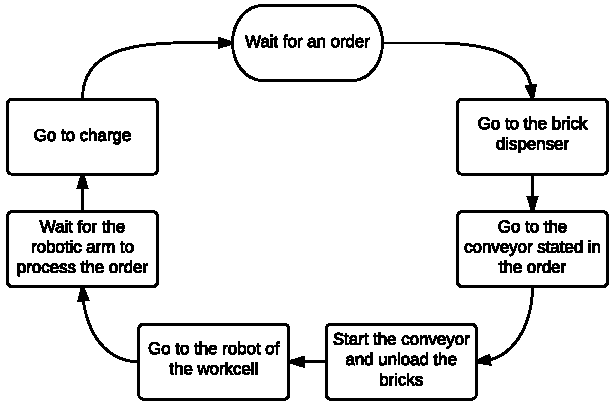
\includegraphics[width=0.75\textwidth]{flow_control}
	\caption{Flow control of the main node in the mobile robot}
	\label{fig:flow_control}
\end{figure}

This process is handled by the \emph{main node}, and this is the highest abstraction level in the control of the robot.
It is responsible of coordinate and actuate a second layer of abstraction which, at the same time, will be responsible of directly actuate the hardware.
The communications between the \emph{main node} an the second layer of abstraction, is shown in the figure \ref{fig:main_connections}.

\begin{figure}[htb]
	\centering
	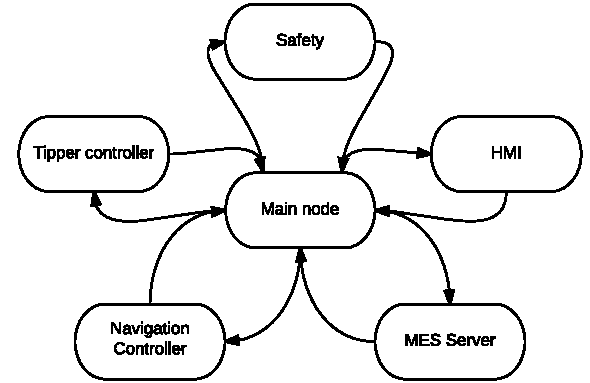
\includegraphics[width=.75\textwidth]{main_connections}
	\caption{Connections of the main node}
	\label{fig:main_connections}
\end{figure}

The main node has also an internal state of the robot represented in three states: \emph{idle}, \emph{auto} and \emph{manual}. 
The mode \emph{idle} means that the robot is not moving or executing any action. 
The mode \emph{auto} means that is processing an order and, consequently, it can be moving. \emph{Manual} stands for when the robot is being moved manually with the HMI. 
The states are intrinsically exclusive and the robot can only be controller manually if the robot is not processing an order.
This avoids the possibility of the user to interfere in the order status increasing the stability and reliability.

The connections are bidirectional and their functions are:
\begin{enumerate}
	\item \textbf{Safety}: Reads the state of the different sensors in the robot that measure the possibility of harm the robot and, if in danger, sends a signal to stops all the actuators.  
	\item \textbf{HMI}: This can change the state of the robot to \emph{auto} to start/continue an order, to \emph{idle} to pause the current order or to \emph{manual} if the user wants to control the robot manually. On the other hand, the main node can tell the HMI (1) its position and (2) the actions being carried out in that moment. This is that in the HMI is shown if the robot is, for example, inside the box and following the line or doing a relative movement.
	\item \textbf{MES server}: The main node reads the order sent and starts the new hierarchy of actions. Also the main node can send messages to the MES in order to activate other agents controlled by this.
	\item \textbf{Navigation controller}: As will be explained in the sections \ref{sec:mr_navigation_controller}, it is responsible of, knowing the current position of the robot, calculate a path to the desired position and perform it. The main node can receive from it when the robot has reached the desired position.
	\item \textbf{Tipper controller}: Handles the position of the tipper assembled in the robot. The controller can talk to the main node to tell when has finished the desired movement.
\end{enumerate}

% section flow_control_overview (end)

